\documentclass[pdftex,10pt,xcolor=svgnames]{beamer}

\mode<presentation>
{
  \usetheme{boxes}
  \usecolortheme[named=MidnightBlue]{structure}
  %\setbeamercolor{normal text}{bg=NavajoWhite!20}
  \usefonttheme{serif}
  \setbeamertemplate{navigation symbols}{}
  % Show frame number and author name in footline
  %\setbeamertemplate{footline}[frame number]
  %\setbeamertemplate{headline}{\scriptsize{\vspace*{0.3cm}\hspace*{0.3cm}\insertframenumber}}
  %\addtobeamertemplate{footline}{\quad\textcolor{gray}{James Lloyd}}{}
  \addtobeamertemplate{frametitle}{\vskip1.5ex}{}
  % Set frame titles in small capitals
  \setbeamerfont{frametitle}{shape=\scshape,family=\rmfamily}
  %\setbeamercolor{frametitle}{bg=gray!60!white,fg=black}
  \setbeamercolor{frametitle}{fg=black}
  % Alerted text: blue (uncomment second line if theme sets alerted text to bold)
  \setbeamercolor{alerted text}{fg=blue}
  %\setbeamerfont*{alerted text}{}
  \setbeamertemplate{bibliography item}[text] %{\hbox{\donotcoloroutermaths$\blacktriangleright$}}
  \setbeamertemplate{bibliography entry title}{}
  \setbeamertemplate{bibliography entry author}{}
  \setbeamertemplate{bibliography entry note}{}
  \setbeamertemplate{bibliography entry location}{}

}
\usepackage[english]{babel}
\usepackage[latin1]{inputenc}
\usepackage{times}
\usepackage[T1]{fontenc}
\usepackage{hyperref}
\usepackage{multimedia}
\usepackage{eepic}
\usepackage{graphicx}
%\usepackage[nohug]{latexinclude/diagrams}
\usepackage{tikz}
\usetikzlibrary{calc}

%% \newcommand{\footlineextra}[1]{
%%     \begin{tikzpicture}[remember picture,overlay]
%%         \node[yshift=1.5ex,anchor=south east] at (current page.south east)
%% {#1};
%%     \end{tikzpicture}
%% }

\newcommand{\footlineextra}[1]{
    \begin{tikzpicture}[remember picture,overlay]
        \node[xshift=-5ex,yshift=-0.5ex,anchor=south east] at (current page.south east)
             {\mbox{\tiny \textcolor{MidnightBlue}{#1}}};
    \end{tikzpicture}
}

\def\sectionframe#1{
  {
    \setbeamertemplate{footline}{\empty}
    \begin{frame}{}
      \begin{center}
        \huge\sc #1
      \end{center}
    \end{frame}
  }
}



\usecolortheme{default}
\xdefinecolor{Black}{rgb}{0,0,0}
\xdefinecolor{White}{rgb}{1,1,1}
\xdefinecolor{DarkBlue}{rgb}{0,0,.7}
\xdefinecolor{DarkRed}{rgb}{.7,0,0}
\xdefinecolor{Red}{rgb}{.85,0,0}
\xdefinecolor{DarkGreen}{rgb}{0,.7,0}
\xdefinecolor{DarkMagenta}{rgb}{.6,0,.6}
\def\Black{\textcolor{Black}}
\def\White{\textcolor{White}}
\def\Blue{\textcolor{DarkBlue}}
\def\Magenta{\textcolor{DarkMagenta}}
\def\Red{\textcolor{Red}}
\def\Green{\textcolor{DarkGreen}}
\definecolor{camlightblue}{rgb}{0.601 , 0.8, 1}

%%%%%%%%%%%%%%%%%%%%%%%%%%%%%%%%%%%%%%%%%%%%%%%%%%%%%%%%%%
%%%% EDITING HELPER FUNCTIONS  %%%%%%%%%%%%%%%%%%%%%%%%%%%
%%%%%%%%%%%%%%%%%%%%%%%%%%%%%%%%%%%%%%%%%%%%%%%%%%%%%%%%%%

%% NA: needs attention (rough writing whose correctness needs to be verified)
%% TBD: instructions for how to fix a gap ("Describe the propagation by ...")
%% PROBLEM: bug or missing crucial bit 

%% use \fXXX versions of these macros to put additional explanation into a footnote.  
%% The idea is that we don't want to interrupt the flow of the paper or make it 
%% impossible to read because there are a bunch of comments.

%% NA's (and TBDs, those less crucially) should be written so 
%% that they flow with the text.

\definecolor{WowColor}{rgb}{.75,0,.75}
\definecolor{SubtleColor}{rgb}{0,0,.50}

% inline
\newcommand{\NA}[1]{\textcolor{SubtleColor}{ {\tiny \bf ($\star$)} #1}}
\newcommand{\LATER}[1]{\textcolor{SubtleColor}{ {\tiny \bf ($\dagger$)} #1}}
\newcommand{\TBD}[1]{\textcolor{SubtleColor}{ {\tiny \bf (!)} #1}}
\newcommand{\PROBLEM}[1]{\textcolor{WowColor}{ {\bf (!!)} {\bf #1}}}

% as margin notes

\newcounter{margincounter}
\newcommand{\displaycounter}{{\arabic{margincounter}}}
\newcommand{\incdisplaycounter}{{\stepcounter{margincounter}\arabic{margincounter}}}

\newcommand{\fTBD}[1]{\textcolor{SubtleColor}{$\,^{(\incdisplaycounter)}$}\marginpar{\tiny\textcolor{SubtleColor}{ {\tiny $(\displaycounter)$} #1}}}

\newcommand{\fPROBLEM}[1]{\textcolor{WowColor}{$\,^{((\incdisplaycounter))}$}\marginpar{\tiny\textcolor{WowColor}{ {\bf $\mathbf{((\displaycounter))}$} {\bf #1}}}}

\newcommand{\fLATER}[1]{\textcolor{SubtleColor}{$\,^{(\incdisplaycounter\dagger)}$}\marginpar{\tiny\textcolor{SubtleColor}{ {\tiny $(\displaycounter\dagger)$} #1}}}


%% For submission, make all render blank.
%\renewcommand{\LATER}[1]{}
%\renewcommand{\fLATER}[1]{}
%\renewcommand{\TBD}[1]{}
%\renewcommand{\fTBD}[1]{}
%\renewcommand{\PROBLEM}[1]{}
%\renewcommand{\fPROBLEM}[1]{}
%\renewcommand{\NA}[1]{#1}  %% Note, NA's pass through!

\usepackage{alltt}
\usepackage{psfrag}
\usepackage{pstool}
\usepackage{multicol}
\usepackage{tabularx}
\usepackage{preamble}

\def\newarrow{\mbox{\begin{tikzpicture}
             \useasboundingbox{(-3pt,-4.5pt) rectangle (19pt,1pt)};
             \draw[->] (0,-0.07)--(17pt,-0.07);\end{tikzpicture}}}
             
\setbeamertemplate{background} {
\includegraphics[width=\paperwidth,height=\paperheight,keepaspectratio]{2010-PES-PPT-Template-v2007.pdf}}

\title[] % (optional, use only with long paper titles)
{GEFCom2012 Hierarchical load forecasting:\\Gradient boosting machines and Gaussian processes}

\author % (optional, use only with lots of authors)
{James Robert Lloyd}
% - Use the \inst{?} command only if the authors have different
%   affiliation.

\institute[] % (optional, but mostly needed)
{Machine Learning Group,\\Department of Engineering,\\University of Cambridge}
% - Use the \inst command only if there are several affiliations.
% - Keep it simple, no one is interested in your street address.

\date % (optional)
{July 2013}

\subject{Talks}

\usetikzlibrary{shapes.geometric,arrows,chains,matrix,positioning,scopes}
 \makeatletter
 \tikzset{join/.code=\tikzset{after node path={%
       \ifx\tikzchainprevious\pgfutil@empty\else(\tikzchainprevious)%
       edge[every join]#1(\tikzchaincurrent)\fi}}
 }
 \tikzset{>=stealth',every on chain/.append style={join},
   every join/.style={->}
 }

\tikzstyle{mybox} = [draw=none, rectangle]
\usepackage{ifthen}
\usepackage{booktabs}

% Custom definitions
\def\simiid{\sim_{\mbox{\tiny iid}}}
\def\ie{i.e.\ }
\def\eg{e.g.\ }

%%%%
% Paper specific stuff
%%%%

\begin{document}

\small
%% { 
%%   \setbeamertemplate{footline}{\empty}
%%   \begin{frame}
%%     \titlepage
%%   \end{frame}
%% }
%\renewcommand{\inserttotalframenumber}{11}

%\theoremstyle{plain}

\def\ie{i.e.\ }
\def\eg{e.g.\ }
\def\indicator{\mathbb{I}}
\def\mean#1{\mathbb{E}[#1]}
\def\bigmean#1{\mathbb{E}\bigl[#1\bigr]}
\def\Bigmean#1{\mathbb{E}\Bigl[#1\Bigr]}
\def\cyl{\mathcal{Z}}
\def\eqae{=_{\mbox{\tiny a.e.}}}
\def\wrt{w.r.t.\ }
\def\ae{a.e.\ }
\def\equas{=_{\mbox{\tiny a.s.}}}
\def\equae{=_{\mbox{\tiny a.e.}}}
\def\iid{i.i.d.\ }
\def\Iid{I.i.d.\ }
%\def\inclusion{\jmath}
\def\inclusion{\mathcal{J}}
\def\inclusionX{\inclusion_{\xspace}}
\def\wstar{weak$^{\ast}$ }
% Symmetric difference
\def\symmdiff{\!\vartriangle\!}


% Indices

\def\indI{\mbox{\tiny I}}
\def\indJ{\mbox{\tiny J}}
\def\indK{\mbox{\tiny K}}
\def\indJI{\mbox{\tiny J$\setminus$I}}
\def\indE{\mbox{\tiny E}}
\def\indF{\mbox{\tiny F}}
\def\indD{\mbox{\tiny D}}
\def\indi{\mbox{\tiny{\{i\}}}}
\def\ind#1{\mbox{\tiny #1}}
\def\power{\mathcal{F}}
\def\powerD{\power(D)}
\def\powerE{\power(E)}
\def\powerL{\power(L)}
\def\parts{\mathcal{H}}
\def\partsQ{\parts(\mathcal{Q})}
\def\partsn{\parts[n]}
\def\partsN{\parts_{\infty}(\mathbb{N})}

% Spaces

\def\abstspace{\Omega}
\def\xspace{\mathcal{X}}
\def\yspace{\mathcal{Y}}
\def\tspace{\mathcal{T}}
\def\xspaceI{\xspace_{\indI}}
\def\xspaceJ{\xspace_{\indJ}}
\def\xspaceD{\xspace_{\indD}}
\def\xspaceE{\xspace_{\indE}}
\def\tspaceI{\tspace_{\indI}}
\def\tspaceJ{\tspace_{\indJ}}
\def\tspaceD{\tspace_{\indD}}
\def\tspaceE{\tspace_{\indE}}
\def\txspace{\tilde{\xspace}}
\def\yspaceI{\yspace_{\indI}}
\def\yspaceJ{\yspace_{\indJ}}
\def\yspaceD{\yspace_{\indD}}
\def\yspaceE{\yspace_{\indE}}
\def\txspace{\tilde{\xspace}}
\def\ttspace{\tilde{\tspace}}
\def\xI{x_{\indI}}
\def\xJ{x_{\indJ}}
\def\xD{x_{\indD}}
\def\xE{x_{\indE}}
\def\tImage{\Gamma}
\def\simp{\triangle}
\def\simpI{\simp_{\indI}}
\def\simpJ{\simp_{\indJ}}

\def\AI{A_{\indI}}
\def\AJ{A_{\indJ}}
\def\AD{A_{\indD}}
\def\AE{A_{\indE}}


%Space of Prob Measures
\def\pMeas{M}
%Space of Contents
\def\fMeas{N}
%Space of cont fcts
\def\cfspace{C}
%Hilbert space
\def\hilbert{\mathcal{L}^2}


\def\borelV{\borel_{V}}

% Set systems

\def\borel{\mathcal{B}}
\def\top{\mbox{Top}}

\def\borelI{\borel_{\indI}}
\def\borelJ{\borel_{\indJ}}
\def\borelD{\borel_{\indD}}
\def\borelE{\borel_{\indE}}
\def\tborel{\tilde{\borel}}
\def\abstfield{\mathcal{A}}
\def\field{\mathcal{C}}
\def\fieldI{\field_{\indI}}
\def\fieldJ{\field_{\indJ}}
\def\fieldK{\field_{\indK}}
\def\fieldD{\field_{\indD}}
\def\fieldE{\field_{\indE}}
\def\tfield{\tilde{\mathcal{C}}}
\def\Sfield{\mathcal{S}}
\def\SfieldI{\mathcal{S}_{\indI}}
\def\SfieldJ{\mathcal{S}_{\indJ}}
\def\SfieldD{\mathcal{S}_{\indD}}
\def\tSfield{\tilde{\mathcal{S}}}
\def\borelx{\borel_x}
\def\tborelx{\tborel_x}
\def\borelgamma{\tborel_{\tImage}}
%\def\borelth{\borel_{\theta}}
\def\borely{\borel_{y}}
%\def\borelT{\borel_t}
\def\borelT{\borel_{\tspace}}
\def\borelS{\borel_s}
\def\topI{\top_{\indI}}
\def\topJ{\top_{\indJ}}
\def\topD{\top_{\indD}}
\def\topE{\top_{\indE}}
\def\topV{\top_V}
\def\topws{\top_{\text{ws}}}
\def\topcc{\top_{\text{c}}}
\def\borelXI{\borel(\xspaceI)}
\def\borelXD{\borel(\xspaceD)}
\def\tborelX{\borel(\txspace)}
\def\borelTI{\borel(\tspaceI)}
\def\borelTD{\borel(\tspaceD)}
\def\tborelT{\borel(\ttspace)}


% Maps

\def\XI{X_{\indI}}
\def\Xi{X_{\ind{i}}}
\def\Xj{X_{\ind{j}}}
\def\ThetaI{\Theta_{\indI}}
\def\XJ{X_{\indJ}}
\def\ThetaJ{\Theta_{\indJ}}
\def\XD{X_{\indD}}
\def\ThetaD{\Theta_{\indD}}
\def\XE{X_{\indE}}
\def\ThetaE{\Theta_{\indE}}
\def\tX{\tilde{X}}
\def\tTheta{\tilde{\Theta}}

\def\SI{S_{\indI}}
\def\TI{T_{\indI}}

\def\rest{\phi}
\def\restD{\rest_{\indD}}
\def\restI{\rest_{\indI}}
\def\restJ{\rest_{\indJ}}
\def\restDI{\rest^{\indD}_{\indI}}
\def\inclusionD{\inclusion_{\indD}}
\def\inclusionE{\inclusion_{\indE}}
\def\projector{\mbox{pr}}
\def\projectorD{\projector_{\indD}}
\def\projectorI{\projector_{\indI}}
\def\projectorJI{\pi_{\indJ\indI}}
\def\indicator{\mathbb{I}}

% Projective systems

\def\po{\preceq}
\def\famD#1{{\lbrace #1 \rbrace}_{\indD}}
\def\famE#1{{\lbrace #1 \rbrace}_{\ind{I$\in$}\indE}}
\def\fJI{f_{\indJ\indI}}
\def\fKI{f_{\indK\indI}}
\def\fKJ{f_{\indK\indJ}}
\def\fII{f_{\indI\indI}}
\def\fI{f_{\indI}}
\def\fJ{f_{\indJ}}
\def\fK{f_{\indK}}
\def\fD{f_{\indD}}
\def\fDI{f^{\indD}_{\indI}}
\def\fDK{f^{\indD}_{\indK}}
\def\gJI{g_{\indJ\indI}}
\def\gI{g_{\indI}}
\def\gJ{g_{\indJ}}
\def\gD{g_{\indD}}
\def\hJI{h_{\indJ\indI}}
\def\hI{h_{\indI}}
\def\hJ{h_{\indJ}}
\def\hE{h_{\indE}}
\def\plim{\varprojlim}

% Measure and Conditionals

\def\abstmeasure{\mathbb{P}}
\def\P{P}
\def\PI{P_{\indI}}
\def\PJ{P_{\indJ}}
\def\PD{P_{\indD}}
\def\PE{P_{\indE}}
\def\PX{P_{\mbox{X}}}
\def\PTh{P_{\mbox{\Theta}}}
\def\PXI{P_{\XI}}
\def\PThI{P_{\mbox{\Theta}}}
\def\PXJ{P_{\mbox{X}}}
\def\PThJ{P_{\mbox{\Theta}}}
\def\PXD{P_{\mbox{X}}}
\def\PThD{P_{\mbox{\Theta}}}
\def\PXE{P_{\mbox{X}}}
\def\PThE{P_{\mbox{\Theta}}}
\def\tP{\tilde{P}}
\def\tPX{\tilde{P}_X}
\def\tPTh{\tilde{P}_{\Theta}}







\def\SI{S_{\indI}}
\def\SJ{S_{\indJ}}

\def\tk{\tilde{k}}
\def\kI{k_{\indI}}

\def\postkernel{k}
\def\indctr{\mathbbm{1}}
\def\sp#1{\left<#1\right>}


%Mallows
\def\Sr{\mathbb{S}_r}
\def\Sinf{\mathbb{S}_{\infty}}
\def\Sbar{\bar{\mathbb{S}}}
\def\DP#1{\mbox{DP}\left( #1 \right)}
\def\GP#1{\mbox{GP}\left( #1 \right)}
\def\x{\mathbf{x}}
\def\y{\mathbf{y}}



\def\tyspace{\tilde{\yspace}}
\def\tF{\tilde{F}}
\def\tT{\tilde{T}}
\def\tmodel{\tilde{\model}}
\def\tnu{\tilde{\nu}}


\def\PTheta{P^{\theta}}
\def\FTheta{F^{\theta}}
\def\TTheta{T^{\theta}}
\def\borelY{\borel_{\yspace}}

\def\PX{P^{x}}
\def\PXI{\PX_{\indI}}
\def\PXJ{\PX_{\indJ}}
\def\PXD{\PX_{\indD}}
\def\PThetaI{\PTheta_{\indI}}
\def\PThetaD{\PTheta_{\indD}}
\def\YI{Y_{\indI}}
\def\YJ{Y_{\indJ}}
\def\YD{Y_{\indD}}
\def\Tn{T^{(n)}}
\def\indexspace{\mathcal{W}}
\def\tyspace{\tilde{\yspace}}
\def\tY{\tilde{Y}}
\def\inclusionT{\inclusion_{\tspace}}
\def\tPTheta{\tilde{P}^{\theta}}
\def\tTn{\tilde{T}^{(n)}}
\def\inclusionY{\inclusion_{\yspace}}

\def\tyspace{\tilde{\yspace}}
\def\tF{\tilde{F}}
\def\tT{\tilde{T}}
\def\tmodel{\tilde{\model}}
\def\tnu{\tilde{\nu}}
\def\tOmega{\tilde{\abstspace}}
\def\tabstmeasure{\tilde{\abstmeasure}}
\def\model{\mathcal{P}}

\def\tf{\tilde{f}}
\def\tx{\tilde{x}}
\def\Dom{\mbox{Dom}}
\def\ty{\tilde{y}}

%Extra stuff - to be integrated in the future

\newcommand{\eqd}{\overset{\,_{\!d}}{=}}
\newcommand{\defn}[1]{\emph{#1}}

\newcommand{\Law}{\mathcal{L}}

\def\given{\,|\,}

\newcommand{\NonNegInts}{\mathbb{Z}_+}
\newcommand{\Nats}{\mathbb{N}}
\newcommand{\Rationals}{\mathbb{Q}}
\newcommand{\Reals}{\mathbb{R}}

\newcommand{\as}{\textrm{a.s.}}

\def\[#1\]{\begin{align}#1\end{align}}
\newcommand{\defas}{:=}

\newcommand{\Normal}{\mathcal{N}}
\newcommand{\dist}{\ \sim\ }

\newcommand{\kernel}{\kappa}
\newcommand{\kernelmatrix}{K}
\newcommand{\scalefactor}{s}
\newcommand{\lengthscale}{\ell}
\newcommand{\targets}{T}
\newcommand{\noise}{\sigma_\targets}
\newcommand{\pseudopoints}{\eta}
\newcommand{\inputpoints}{\xi}
\newcommand{\covhyppar}{\psi}
\newcommand{\logistic}{\phi}

\newcommand{\CompOrder}{\mathcal{O}}

\newtheorem{thm}{Theorem}%[section]
\newtheorem{lem}[thm]{Lemma}
\newtheorem{prop}[thm]{Proposition}
\newtheorem{cor}[thm]{Corollary}

\theoremstyle{definition}
\newtheorem{definition}[thm]{Definition}%[section]
\newtheorem{conj}{Conjecture}[section]
\newtheorem{exmp}{Example}[section]
\newtheorem{rem}[thm]{Remark}

\theoremstyle{remark}
%\newtheorem{rem}{Remark}
\newtheorem{note}{Note}
\newtheorem{case}{Case}

\def\Uniform{\mbox{\rm Uniform}}
\def\Bernoulli{\mbox{\rm Bernoulli}}
\def\ie{i.e.\ }
\def\eg{e.g.\ }
\def\etc{etc.\ }
\def\iid{i.i.d.\ }
\def\simiid{\sim_{\mbox{\tiny iid}}}
\def\eqdist{\stackrel{\mbox{\tiny d}}{=}}
\def\GP{\mathcal{GP}}
\def\Transpose{^\textrm{T}}


\begin{frame}
  %\begin{block}{}
    \titlepage
  %\end{block}
  \begin{center}
    {\bf  Thanks to}\\
    Alex Davies\\
    David Duvenaud\\
    Zoubin Ghahramani
  \end{center}
\end{frame}

\begin{frame}{Overview of techniques}
  \begin{block}{Preprocessing}
    %\vspace{\baselineskip}
    \begin{itemize}
      \item Kernel smoothing of temperatures (to remove daily periodicity)
    \end{itemize}
  \end{block}
  \vspace{\baselineskip}
  \begin{block}{Temperature forecasting}
    %\vspace{\baselineskip}
    \begin{itemize}
      \item Gaussian process (GP) regression
    \end{itemize}
  \end{block}
  \vspace{\baselineskip}
  \begin{block}{Load back/forecasting}
    %\vspace{\baselineskip}
    \begin{itemize}
      \item Gradient boosting machine (GBM) regression  - 76\%
      \item Gaussian process (GP) regression - 14\%
      \item Linear regression (benchmark solution) - 10\%
    \end{itemize}
  \end{block}
\end{frame}

\begin{frame}{Performance of Different Components}
  \begin{center}
    \begin{tabular}{lcc|ccc}
      Method &&&&& Validation score\\&&&&&\\
      \hline&&&&&\\
      GBM &&&&& 72,968 \\&&&&&\\
      GP &&&&& 99,787 \\&&&&&\\
      LR &&&&& 112,547 \\&&&&&\\
      \hline&&&&&\\
      Ensemble &&&&& 71,164
    \end{tabular}
  \end{center}
  \begin{itemize}
    \item GBM the best performing method
    \item GP and LR sufficiently uncorrelated with GBM to provide useful components in ensemble
  \end{itemize}
\end{frame}

%\begin{frame}{Notation}
%  \begin{itemize}
%    \item $t$ --- Time
%    \vspace{\baselineskip}
%    \item $T$ --- Temperature
%    \vspace{\baselineskip}
%    \item $S$ --- Kernel smoothed temperature
%    \vspace{\baselineskip}
%    \item $Z$ --- Load
%    \vspace{\baselineskip}
%    \item $f,g$ --- Generic functions
%    \vspace{\baselineskip}
%    \item $\varepsilon$ --- Generic error
%  \end{itemize}
%\end{frame}

\begin{frame}{Main approach - regression on time and temp.}
  \begin{block}{Modelling temperatures and loads as functions of time and temperature}
    \vspace{-1\baselineskip}
    \begin{eqnarray*}
      T(t) & = & f(t, \bar{S}(t)) + \varepsilon^T_t \\
      \\
      Z(t) & = & g(t, T(t), S(t)) + \varepsilon^Z_t \\
    \end{eqnarray*}
    \vspace{-2\baselineskip}
  \end{block}
  \begin{block}{\ie no explicit autoregressive components \eg}
    \vspace{-1\baselineskip}
    \begin{eqnarray*}
      y(t+1) & = & f(y(t)) + \varepsilon_t
    \end{eqnarray*}
  \end{block}
  \begin{block}{Notation}
    $t$ --- Time, $T$ --- Temperature, $S$ --- Smoothed temperature $\bar{S}$ --- Historical average of smoothed temperature, $Z$ --- Load, $f,g$ --- Generic functions, $\varepsilon$ --- Generic error
  \end{block}
\end{frame}

\begin{frame}{GBM regression - overview}
  \begin{block}{Used as a regression `black-box'}
    \begin{itemize}
      \item Bagged and boosted decision trees
      \item Used standard R implementation with most default parameters unchanged
    \end{itemize}
  \end{block}
  \begin{block}{Output}
  	\begin{itemize}
      \item $Z_i$ \ie each load zone modelled in isolation
    \end{itemize}
  \end{block}
  \begin{block}{Inputs}
    \begin{itemize}
      \item Time of day
      \item Time within week
      \item Temperatures (all stations)
      \item Smoothed temperatures (all stations)
    \end{itemize}
  \end{block}
\end{frame}

\begin{frame}{GBM regression - parameter selection}
  \begin{itemize}
    \item Ideally would have performed grid searches over parameter values using cross validated error as metric
    \vspace{\baselineskip}
    \item In practice, partial grid searches combined with intuition, using out of bag errors and validation score on Kaggle
    \vspace{\baselineskip}
    \item 10,000 trees, interaction depth of 3 and shrinkage factor of 0.01 (other values set to defaults of R implementation)
  \end{itemize}
\end{frame}

\begin{frame}{GBM regression - example}
  \vspace{-2\baselineskip}
  \begin{center}
    \begin{tikzpicture}
  \begin{scope}
    \node [mybox] (box){
      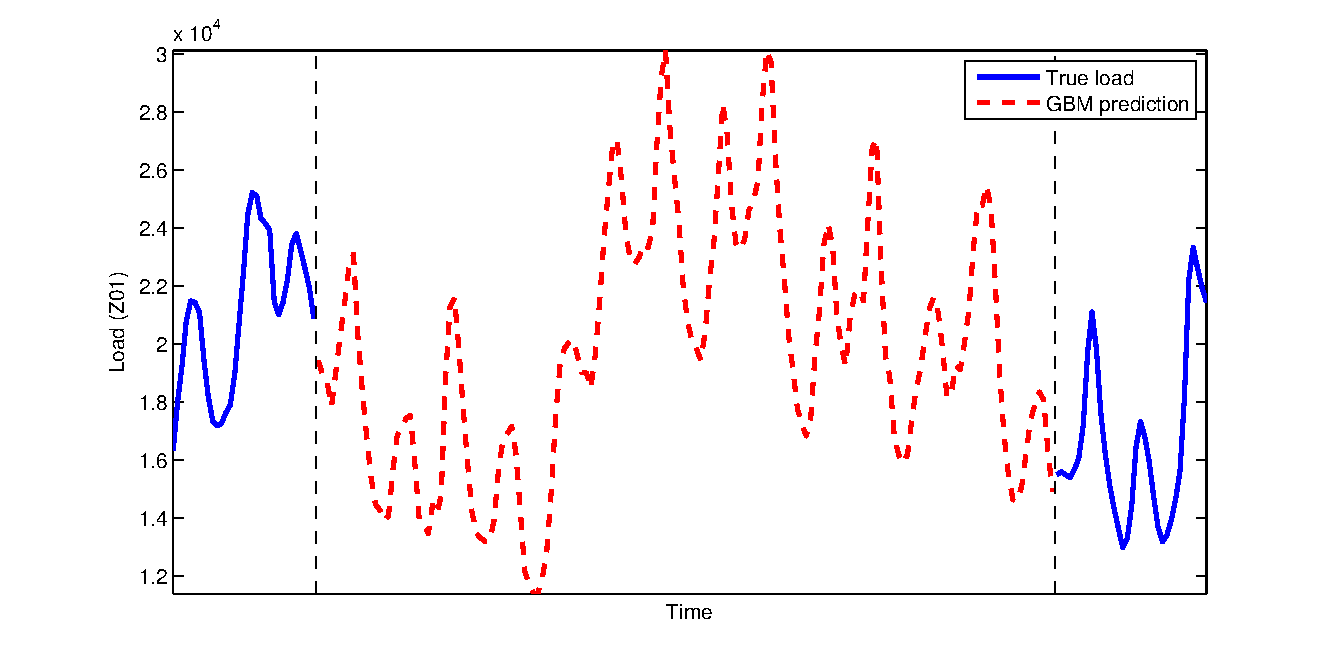
\includegraphics[width=\textwidth]{../include/Z01_pred.pdf}
    };
  \end{scope}
\end{tikzpicture}

  \end{center}
  \vspace{-1\baselineskip}
  Only slight discontinuity between prediction and ground truth despite no explicit modelling assumptions of continuity
\end{frame}

\begin{frame}{Gaussian process regression}
  \begin{itemize}
    \item A Bayesian nonparametric method for regression
    \vspace{\baselineskip}
    \item Places a prior on functions but equivalent to linear regression in an (infinite dimensional) feature space
    \vspace{\baselineskip}
    \item Typically used as a smoothing device by choosing a default \emph{kernel}
    \vspace{\baselineskip}
    \item Data exhibiting high level structure (\eg periodicity) can be modelled using more advanced kernels
  \end{itemize}
\end{frame}

\begin{frame}{Bayesian modelling}
  \begin{block}{Bayes' rule}
    \begin{equation*}
      \mathbb{P}(\textrm{hypothesis}|\textrm{data}) = \frac{\mathbb{P}(\textrm{data}|\textrm{hypothesis})\mathbb{P}(\textrm{hypothesis})}{\mathbb{P}(\textrm{data})}
    \end{equation*}
  \end{block}
  \begin{block}{}
    \begin{itemize}
      \item Bayes' rule follows from basic axioms of probability theory
      \vspace{\baselineskip}
      \item Provides a calculus to update beliefs in response to data
      \vspace{\baselineskip}
      \item Requires the specification of prior beliefs about data - choice of prior is crucial for successful modelling
    \end{itemize}
  \end{block}
\end{frame}

\begin{frame}{Prior on functions}
  \begin{center}
    \begin{tikzpicture}
  \begin{scope}[xshift=0]
    \begin{scope}[yshift=0]
      \node [mybox] (box){
        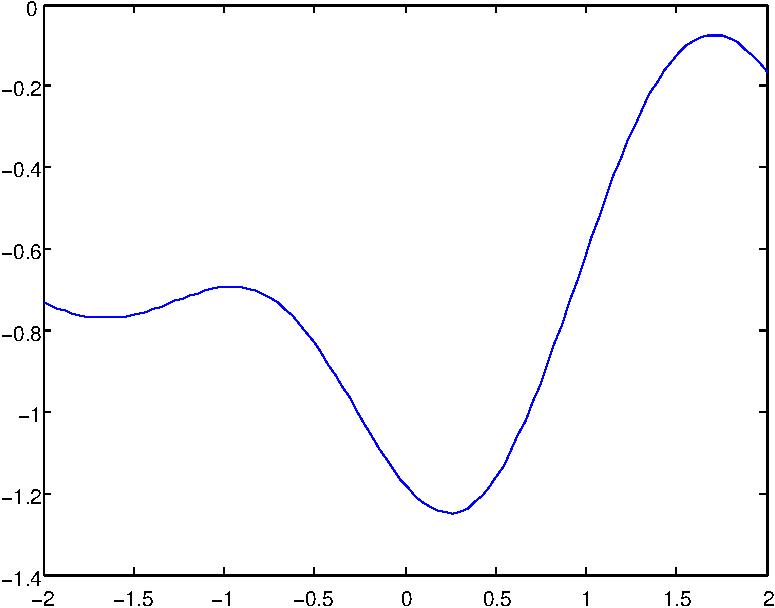
\includegraphics[width=0.35\textwidth]{../include/simple_draw.pdf}
      };
    \end{scope}
    \begin{scope}[yshift=0.35\textwidth]
      \node [mybox] (box){
        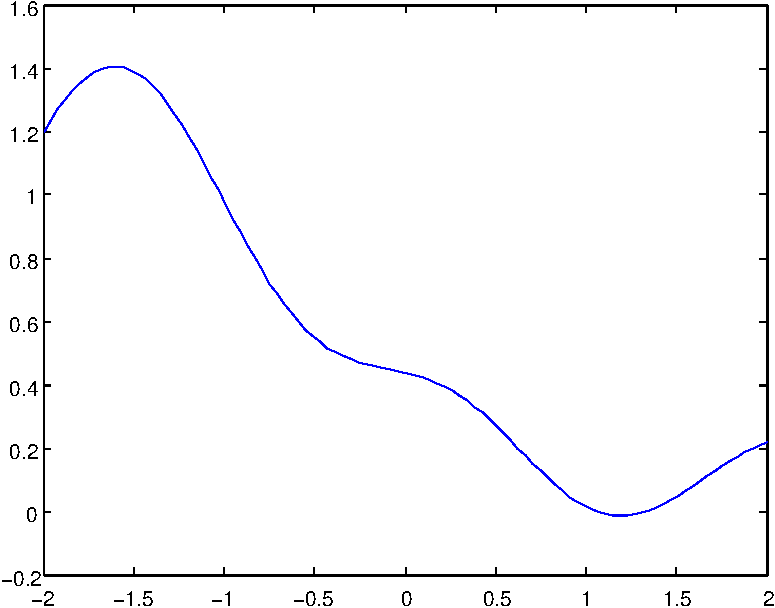
\includegraphics[width=0.35\textwidth]{../include/simple_draw2.pdf}
      };
    \end{scope}
  \end{scope}
  \begin{scope}[xshift=0.5\textwidth]
    \begin{scope}[yshift=0]
      \node [mybox] (box){
        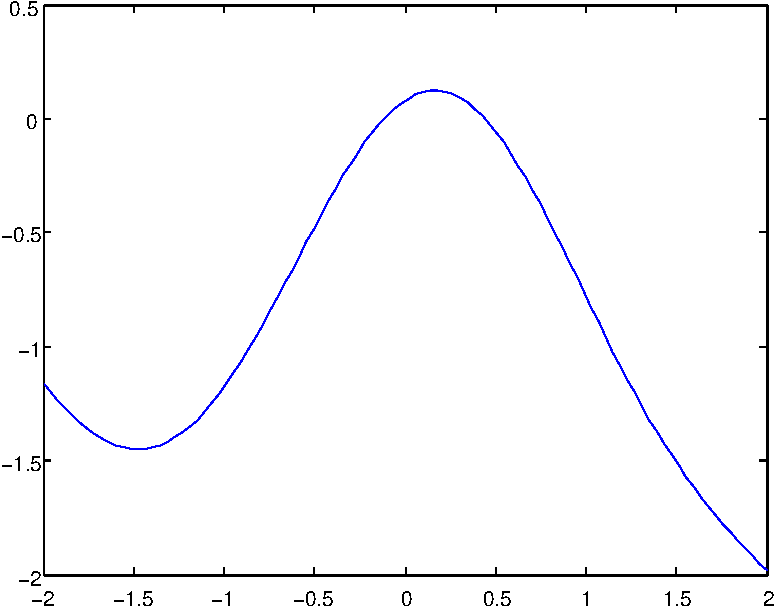
\includegraphics[width=0.35\textwidth]{../include/simple_draw3.pdf}
      };
    \end{scope}
    \begin{scope}[yshift=0.35\textwidth]
      \node [mybox] (box){
        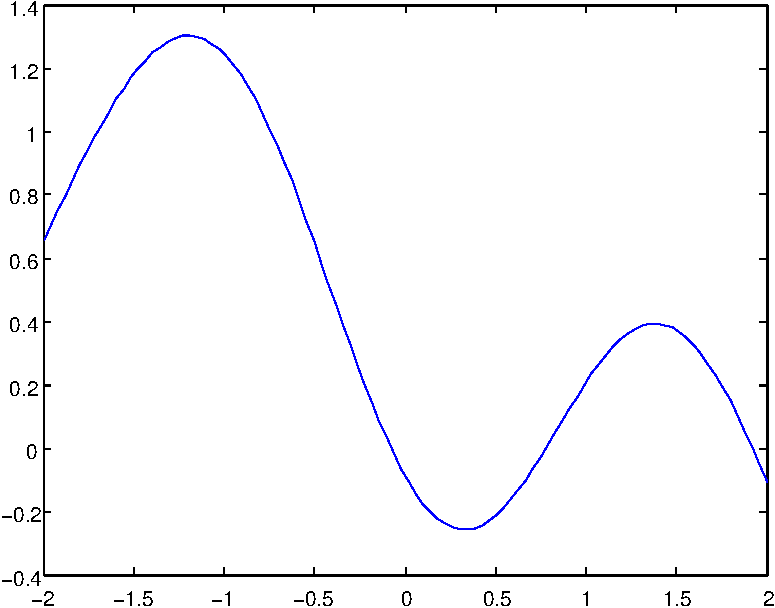
\includegraphics[width=0.35\textwidth]{../include/simple_draw4.pdf}
      };
    \end{scope}
  \end{scope}
\end{tikzpicture}

  \end{center}
\end{frame}

\begin{frame}{Conditional Posterior}
  %\begin{align*}
  %  f(x^*) | X, y \sim \mathcal{N}( & k( x^*, X ) K^{-1} y, \\
  %  & k( x^*, x^* ) - k( x^*, X ) K^{-1} k( X, x^* ) )
  %\end{align*}

  %With SE kernel:
  After observing data, Bayes rule provides a formula by which to update our beliefs about a function
    \begin{figure}
        \includegraphics<1>[width=6cm]{../include/gp_demo/1d_posterior_and_0_data}
        \includegraphics<2>[width=6cm]{../include/gp_demo/1d_posterior_and_1_data}
        \includegraphics<3>[width=6cm]{../include/gp_demo/1d_posterior_and_2_data}
        \includegraphics<4>[width=6cm]{../include/gp_demo/1d_posterior_and_3_data}
        \includegraphics<5>[width=6cm]{../include/gp_demo/1d_posterior_and_4_data}
    \end{figure}
\end{frame}

%\begin{frame}{Need more than just a smoothing device}
%  \begin{center}
%    \begin{tikzpicture}%[transform canvas={scale = 0.9}]
  \begin{scope}[yshift=0\textwidth]
    \begin{scope}[xshift=0\textwidth]
      \node [mybox] at (0, 0) {
        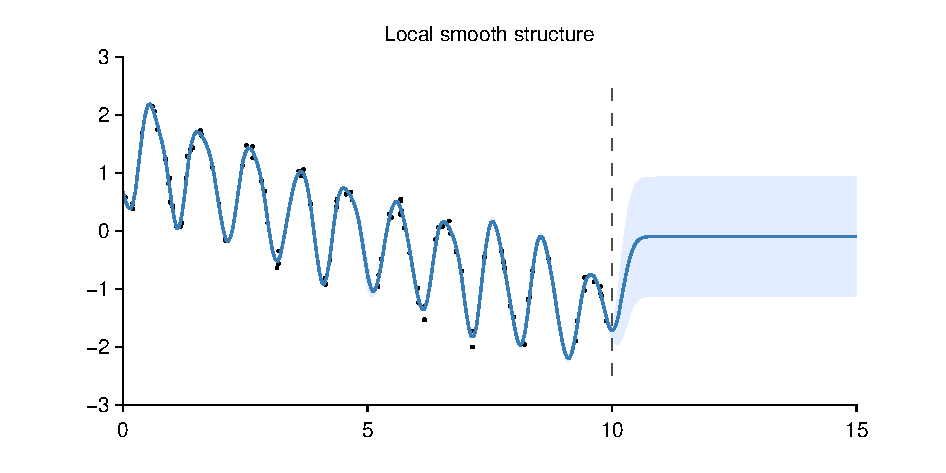
\includegraphics[width=1.0\textwidth]{../include/synth_extrap_bad.pdf}
      };
    \end{scope}
  \end{scope}
\end{tikzpicture}


%  \end{center}
%\end{frame}

%\begin{frame}{Need more than just a smoothing device}
%  \begin{center}
%    \begin{tikzpicture}
  \begin{scope}[xshift=0cm]
    \node [mybox] (box){
      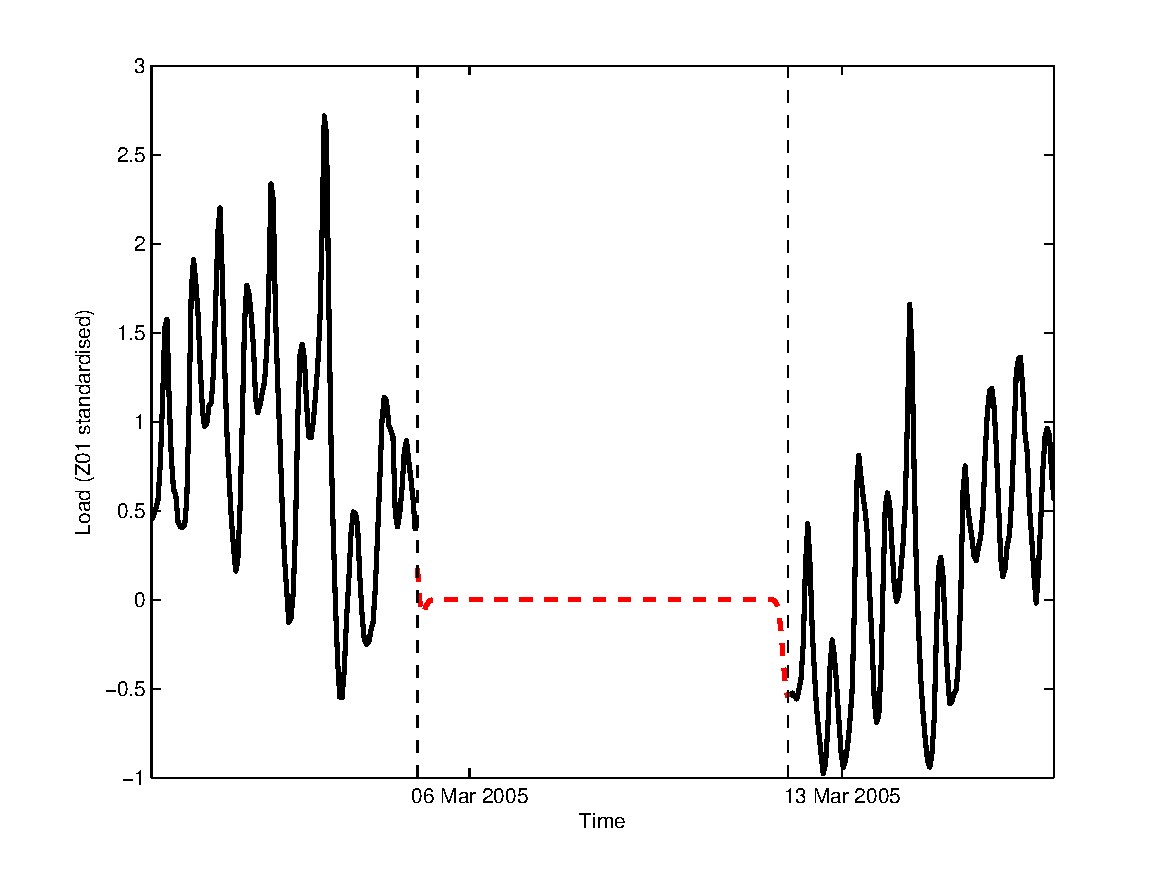
\includegraphics[width=0.9\textwidth]{../include/load_pred_SE.pdf}
    };
  \end{scope}
\end{tikzpicture}

%  \end{center}
%\end{frame}

\begin{frame}{Encoding structural assumptions}
  \begin{itemize}
    \item Gaussian processes typically used as smoothing devices
    \vspace{\baselineskip}
    \item Daily and weekly periodicity assumptions could be encoded by feature engineering as with GBM
    \vspace{\baselineskip}
    \item However, structural assumptions can also be encoded in the \emph{kernel} of a GP
    \begin{itemize}
      \item Using a different method allows predictions to be uncorrelated - very useful for ensembling
    \end{itemize}
  \end{itemize}
\end{frame}

\begin{frame}{Can encode structural assumptions in kernel}
  \begin{itemize} 
	\item Kernel determines the structural properties of a Gaussian process
	\item Many different kinds, with very different properties:
  \end{itemize}
  \newcommand{\fhbig}{1.6cm}
\newcommand{\fwbig}{1.8cm}
\newcommand{\kernpic}[1]{\includegraphics[height=\fhbig,width=\fwbig]{../include/structure_examples/#1}}
\newcommand{\kernpicr}[1]{\rotatebox{90}{\includegraphics[height=\fwbig,width=\fhbig]{../include/structure_examples/#1}}}
\newcommand{\addkernpic}[1]{{\includegraphics[height=\fhbig,width=\fwbig]{../include/additive_multi_d/#1}}}
\newcommand{\largeplus}{\tabbox{{\Large+}}}
\newcommand{\largeeq}{\tabbox{{\Large=}}}
\newcommand{\largetimes}{\tabbox{{\Large$\times$}}}
\begin{figure}[ht]
\centering
\renewcommand{\tabularxcolumn}[1]{>{\arraybackslash}m{#1}}
%\begin{tabular}{m{\fwbig}m{0.01\textwidth}m{\fwbig}m{0.01\textwidth}m{\fwbig}m{\fwbig}m{\fwbig}}
%\begin{tabular}{C{\fwbig}C{\fwbig}C{\fwbig}C{\fwbig}}%{m{\fwbig}m{\fwbig}m{\fwbig}}
\begin{tabularx}{\columnwidth}{XXXX}
%Composite & Draws from \gp{} & \gp{} posterior \\ \toprule
  \kernpic{se_kernel} & \kernpic{se_kernel_draws}
& \kernpic{per_kernel} & \kernpic{per_kernel_draws_s2}
\\
  {\small Squared-exp (\kSE)} & {\small local variation} 
& {\small Periodic (\kPer)} & {\small repeating structure}
\\
  \kernpic{lin_kernel} & \kernpic{lin_kernel_draws}
& \kernpic{rq_kernel} & \kernpic{rq_kernel_draws}
\\
  {\small Linear (\kLin)} & {\small linear functions} 
& {\small Rational-quadratic(\kRQ)} & {\small multi-scale variation}
\end{tabularx}
\end{figure}


\end{frame}

\begin{frame}{Kernels can be composed}
  \begin{itemize} 
	\item Two main operations: adding, multiplying
  \end{itemize}
  \newcommand{\fhbig}{1.6cm}
\newcommand{\fwbig}{1.8cm}
\newcommand{\kernpic}[1]{\includegraphics[height=\fhbig,width=\fwbig]{../include/structure_examples/#1}}
\newcommand{\kernpicr}[1]{\rotatebox{90}{\includegraphics[height=\fwbig,width=\fhbig]{../include/structure_examples/#1}}}
\newcommand{\addkernpic}[1]{{\includegraphics[height=\fhbig,width=\fwbig]{../include/additive_multi_d/#1}}}
\newcommand{\largeplus}{\tabbox{{\Large+}}}
\newcommand{\largeeq}{\tabbox{{\Large=}}}
\newcommand{\largetimes}{\tabbox{{\Large$\times$}}}
\begin{figure}[ht]
\centering
\renewcommand{\tabularxcolumn}[1]{>{\arraybackslash}m{#1}}
%\begin{tabular}{m{\fwbig}m{0.01\textwidth}m{\fwbig}m{0.01\textwidth}m{\fwbig}m{\fwbig}m{\fwbig}}
%\begin{tabular}{C{\fwbig}C{\fwbig}C{\fwbig}C{\fwbig}}%{m{\fwbig}m{\fwbig}m{\fwbig}}
\begin{tabularx}{\columnwidth}{XXXX}
  \kernpic{lin_times_lin} & \kernpic{lin_times_lin_draws} 
& \kernpic{se_times_per} & \kernpic{se_times_per_draws_s7}
\\
  {\small $\kLin \times \kLin$} & {\small quadratic functions}
& {\small $\kSE \times \kPer$} & {\small locally \newline periodic}
\\
%\midrule 
  \kernpic{lin_plus_per} & \kernpic{lin_plus_per_draws}
& \kernpic{se_plus_per} & \kernpic{se_plus_per_draws_s7}
\\
  {\small $\kLin + \kPer$} & {\small periodic with trend}
& {\small $\kSE + \kPer$ } & {\small periodic with noise}
\end{tabularx}
\end{figure}


\end{frame}

%\begin{frame}{Need more than just a smoothing device}
%  \begin{center}
%    \begin{tikzpicture}
  \begin{scope}[xshift=0cm]
    \node [mybox] (box){
      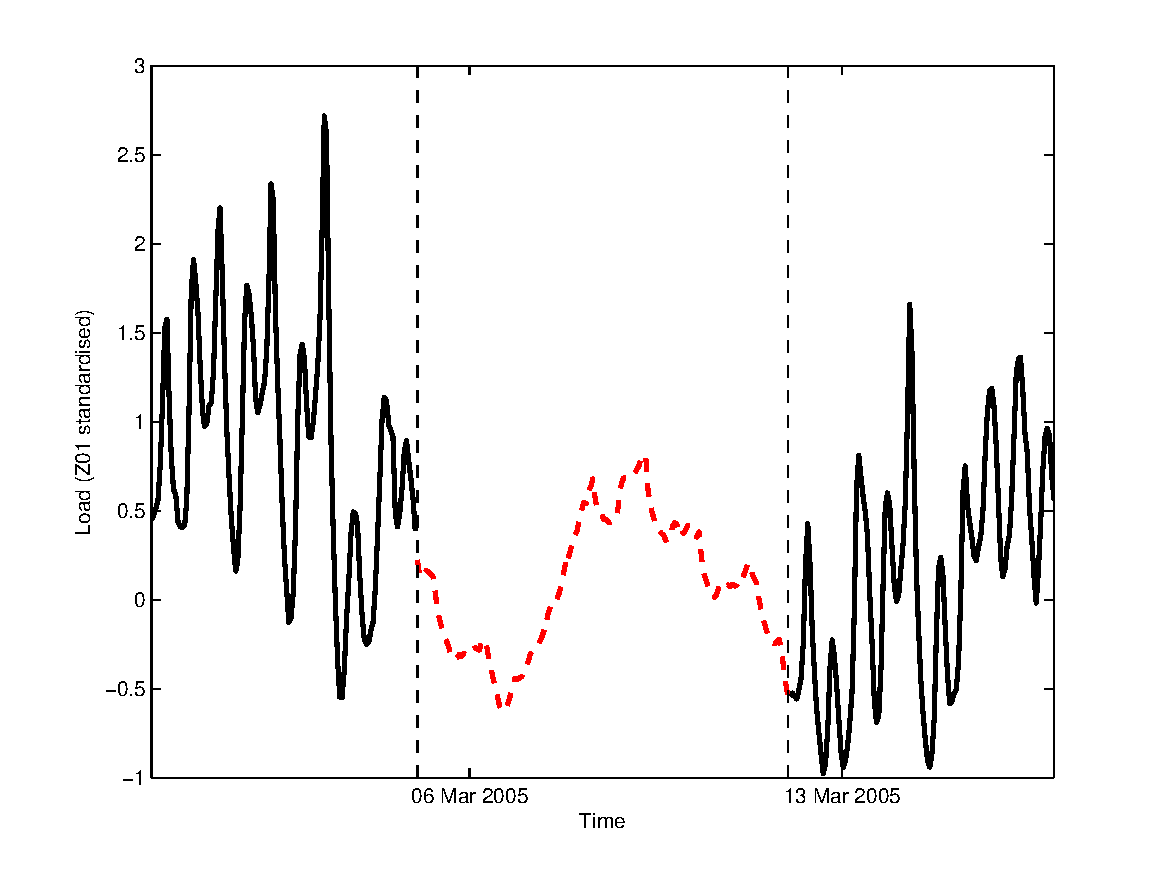
\includegraphics[width=0.5\textwidth]{../include/load_pred_SEard.pdf}
    };
  \end{scope}
  \begin{scope}[xshift=0.5\textwidth]
    \node [mybox] (box){
      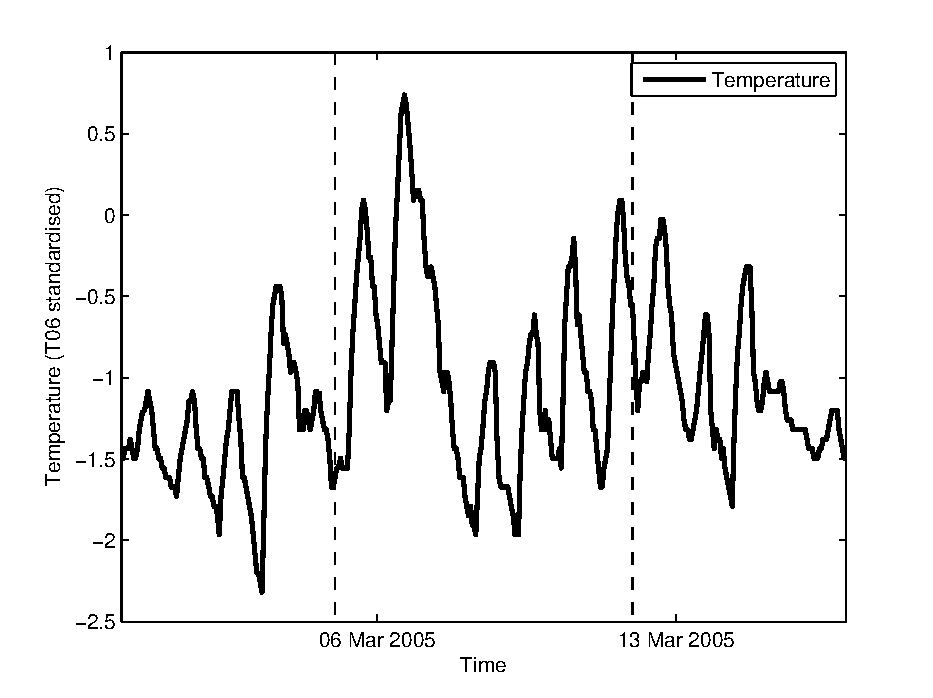
\includegraphics[width=0.5\textwidth]{../include/best_temp.pdf}
    };
  \end{scope}
\end{tikzpicture}

%  \end{center}
%\end{frame}

\begin{frame}{A suitable prior}
  %\begin{itemize}
    %\item Used kernels of the form $\SE_t + \SE_S + \SE_t \times \SE_T \times \Per_t$
    %\item
  Used structured kernel to encode the assumption that
  \begin{eqnarray*}
    \textrm{Load} & = & \textrm{Smooth function of time} +  \\
    & & \textrm{Smooth function of smoothed temperatures} + \\
    & & \textrm{Daily periodicity smoothly changing with time and temperature}
  \end{eqnarray*}
  %\end{itemize}
  \begin{center}
    \begin{tikzpicture}
  \begin{scope}[xshift=0]
    \begin{scope}[yshift=0]
      \node [mybox] (box){
        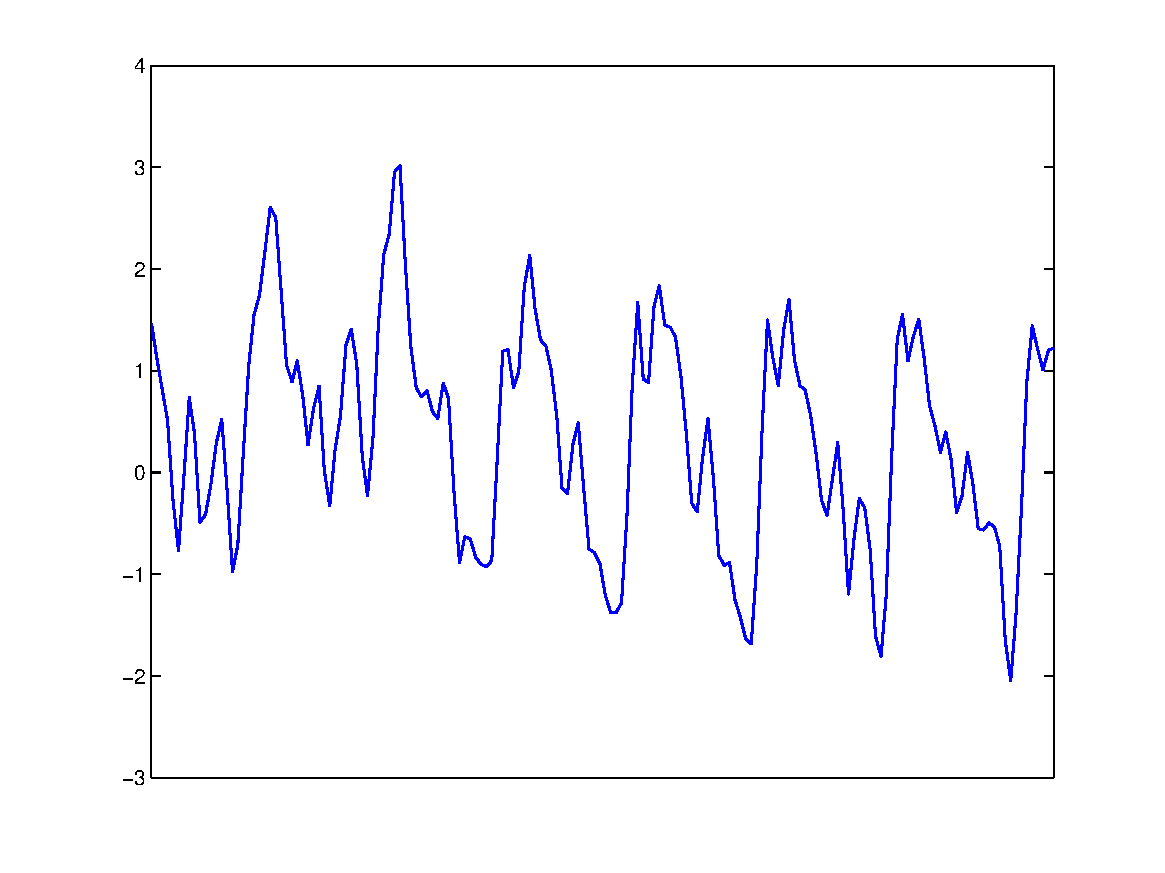
\includegraphics[width=0.40\textwidth]{../include/fancy_kernel_draw1.pdf}
      };
    \end{scope}
  %  \begin{scope}[yshift=0.30\textwidth]
  %    \node [mybox] (box){
  %      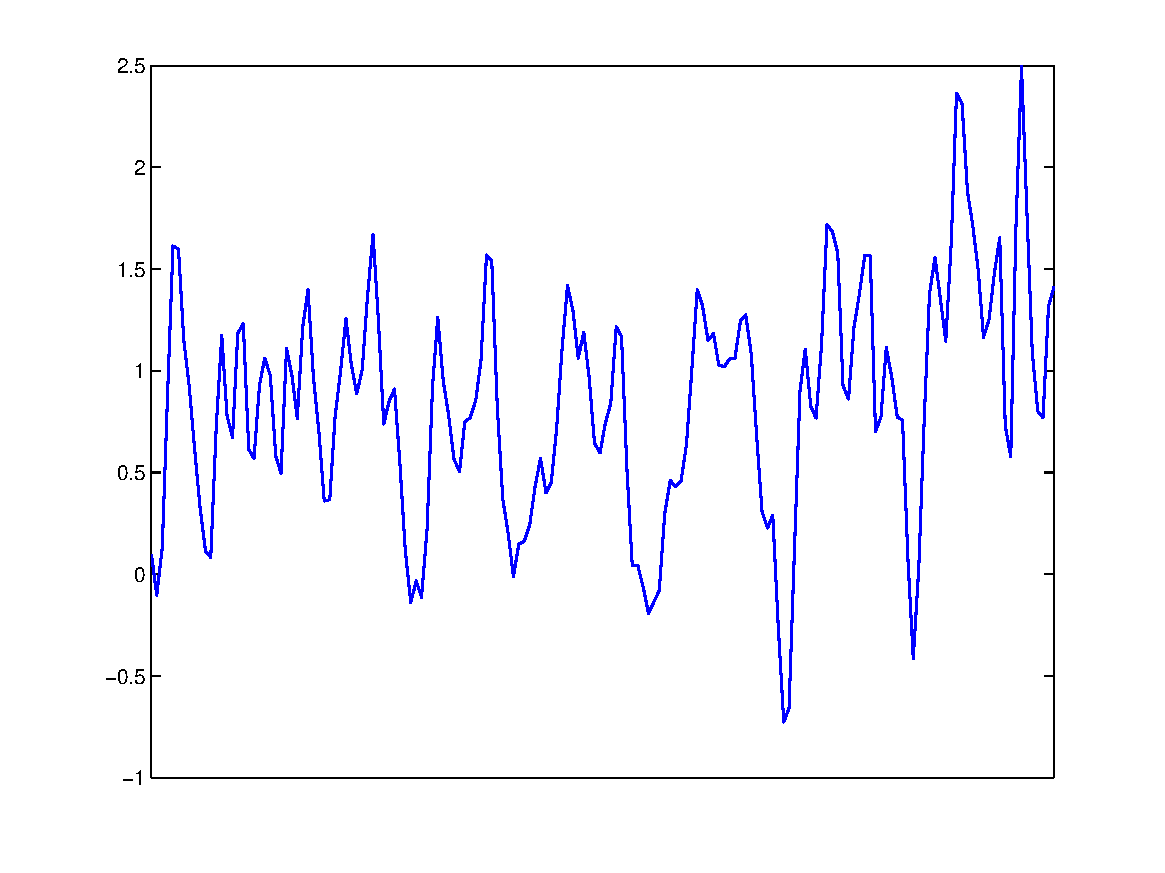
\includegraphics[width=0.40\textwidth]{../include/fancy_kernel_draw2.pdf}
  %    };
  %  \end{scope}
  \end{scope}
  \begin{scope}[xshift=0.5\textwidth]
    \begin{scope}[yshift=0]
      \node [mybox] (box){
        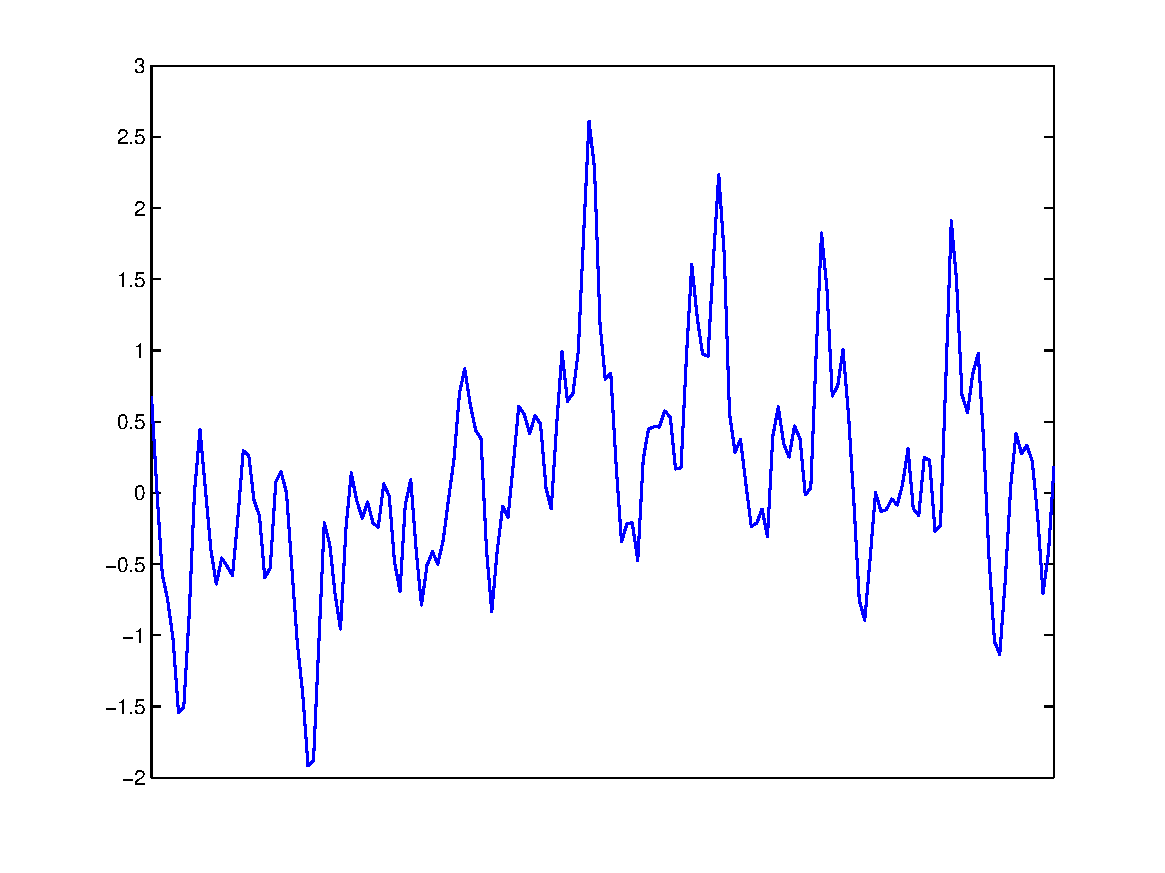
\includegraphics[width=0.40\textwidth]{../include/fancy_kernel_draw3.pdf}
      };
    \end{scope}
  %  \begin{scope}[yshift=0.30\textwidth]
  %    \node [mybox] (box){
  %      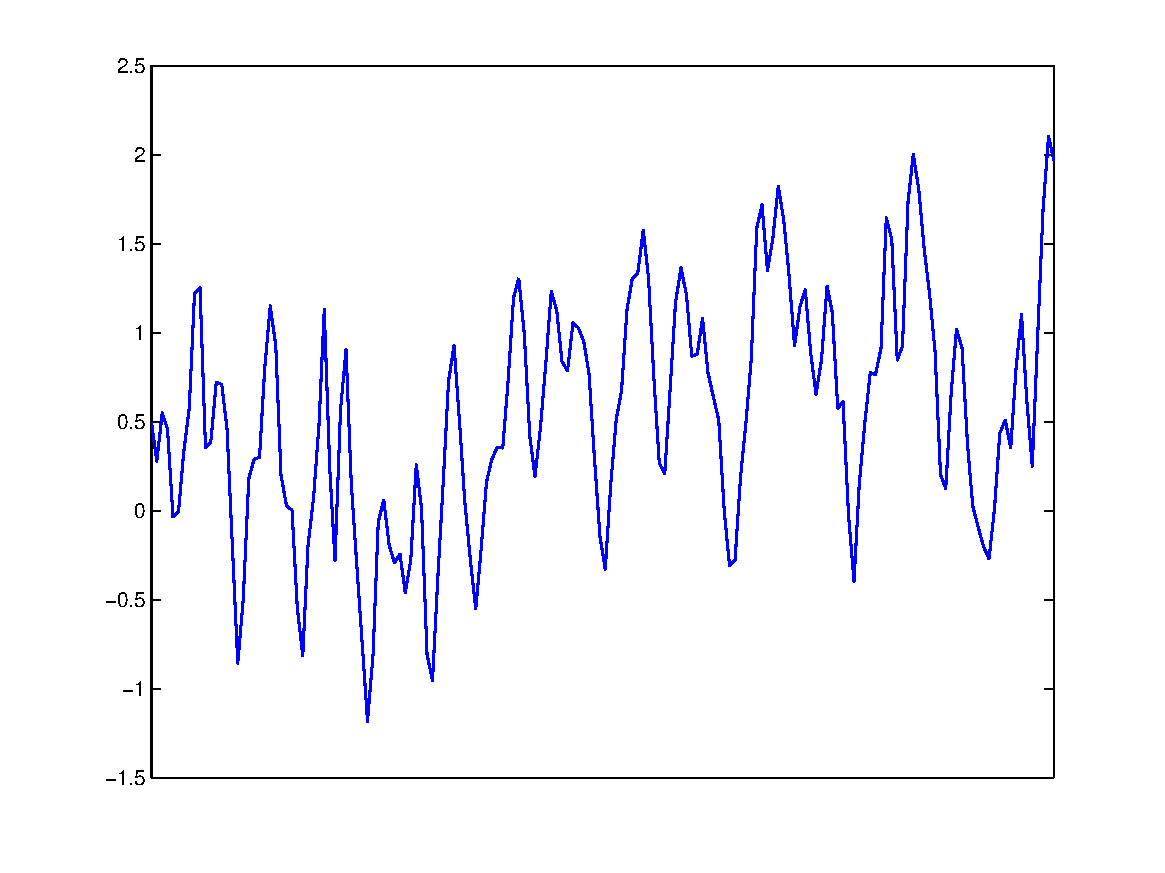
\includegraphics[width=0.40\textwidth]{../include/fancy_kernel_draw4.pdf}
  %    };
  %  \end{scope}
  \end{scope}
\end{tikzpicture}

  \end{center}
\end{frame}

\begin{frame}{GP regression - example}
    \begin{eqnarray*}
    \textrm{Load} & = & \textrm{Smooth function of time} +  \\
    & & \textrm{Smooth function of smoothed temperatures} + \\
    & & \textrm{Daily periodicity smoothly changing with time and temperature}
  \end{eqnarray*}
  \begin{center}
    \begin{tikzpicture}
  \begin{scope}[xshift=0cm]
    \node [mybox] (box){
      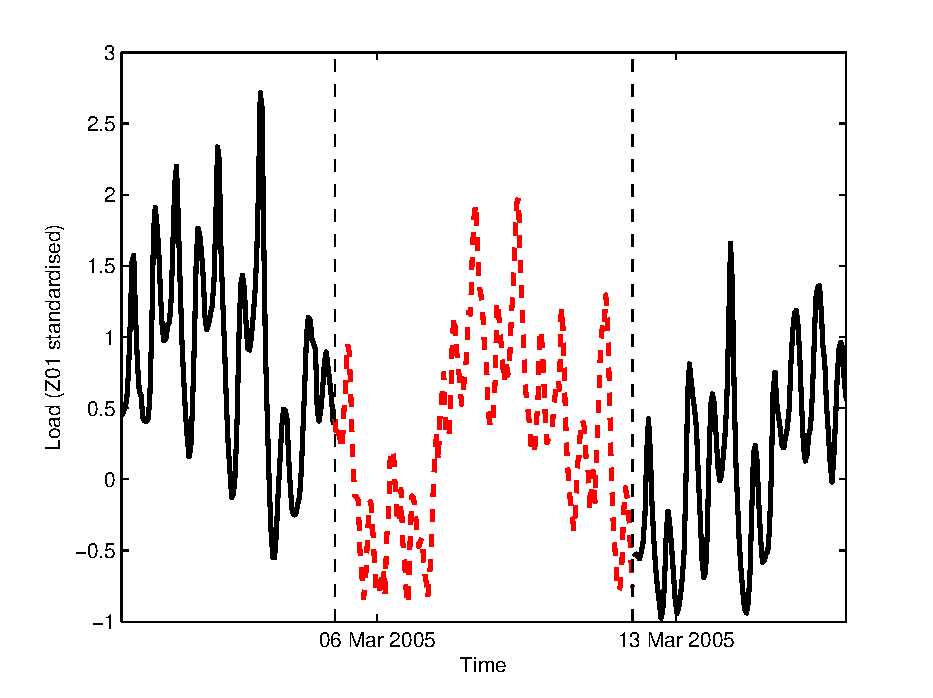
\includegraphics[width=0.5\textwidth]{../include/load_pred.pdf}
    };
  \end{scope}
  \begin{scope}[xshift=0.5\textwidth]
    \node [mybox] (box){
      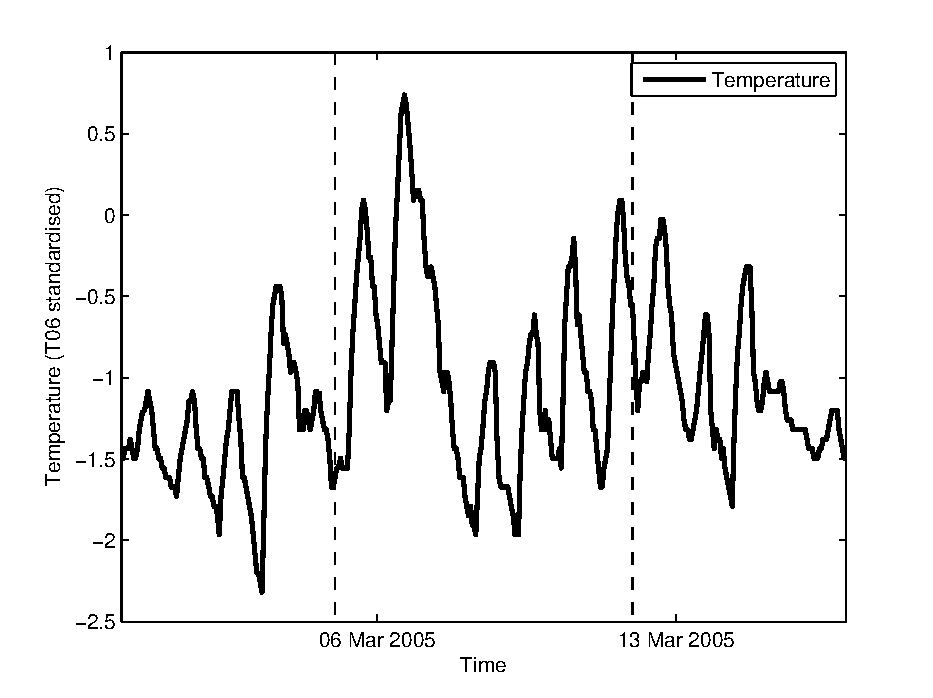
\includegraphics[width=0.5\textwidth]{../include/best_temp.pdf}
    };
  \end{scope}
\end{tikzpicture}

  \end{center}
\end{frame}

%\begin{frame}{GP regression - without periodicity}
%    \begin{eqnarray*}
%    \textrm{Load} & = & \textrm{Smooth function of time} +  \\
%    & & \textrm{Smooth function of temperatures} + \\
%    & & \textrm{Smooth function of smoothed temperatures}
%  \end{eqnarray*}
%  \begin{center}
%    \begin{tikzpicture}
  \begin{scope}[xshift=0cm]
    \node [mybox] (box){
      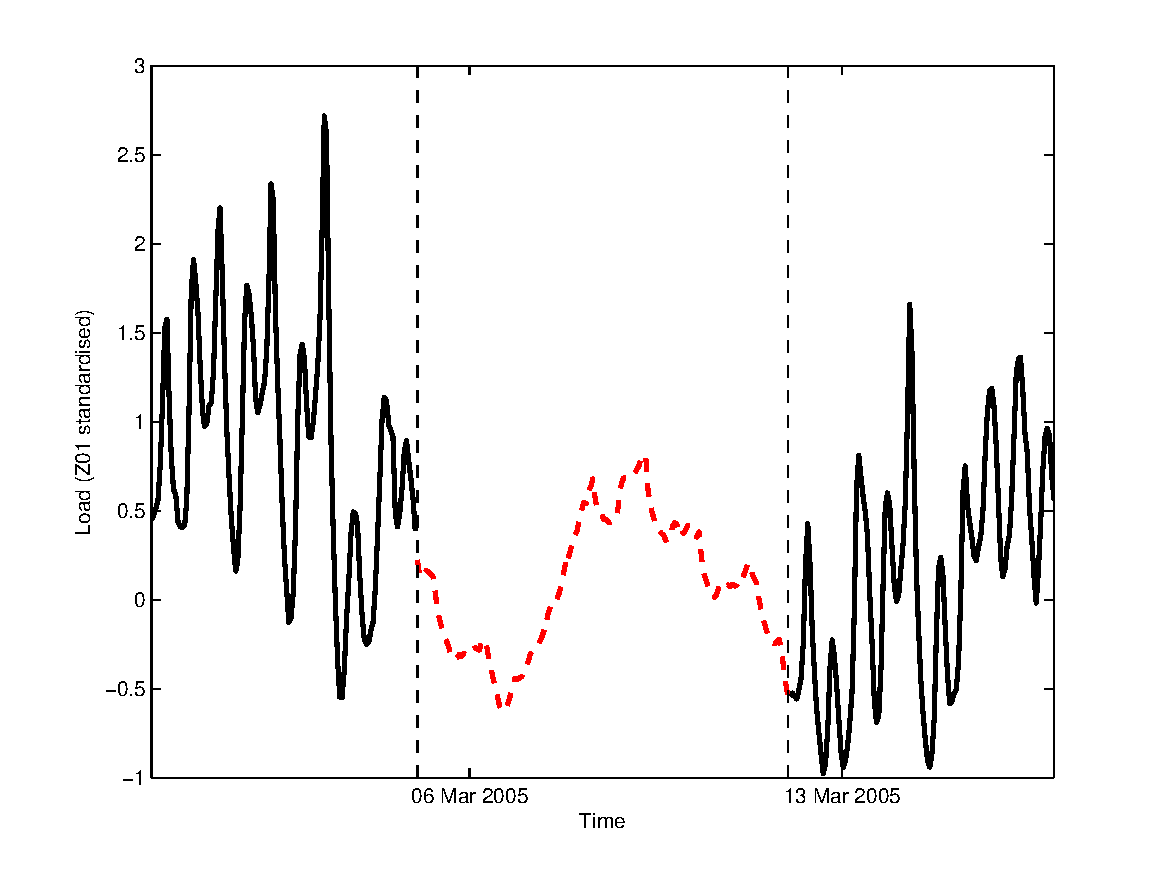
\includegraphics[width=0.5\textwidth]{../include/load_pred_SEard.pdf}
    };
  \end{scope}
  \begin{scope}[xshift=0.5\textwidth]
    \node [mybox] (box){
      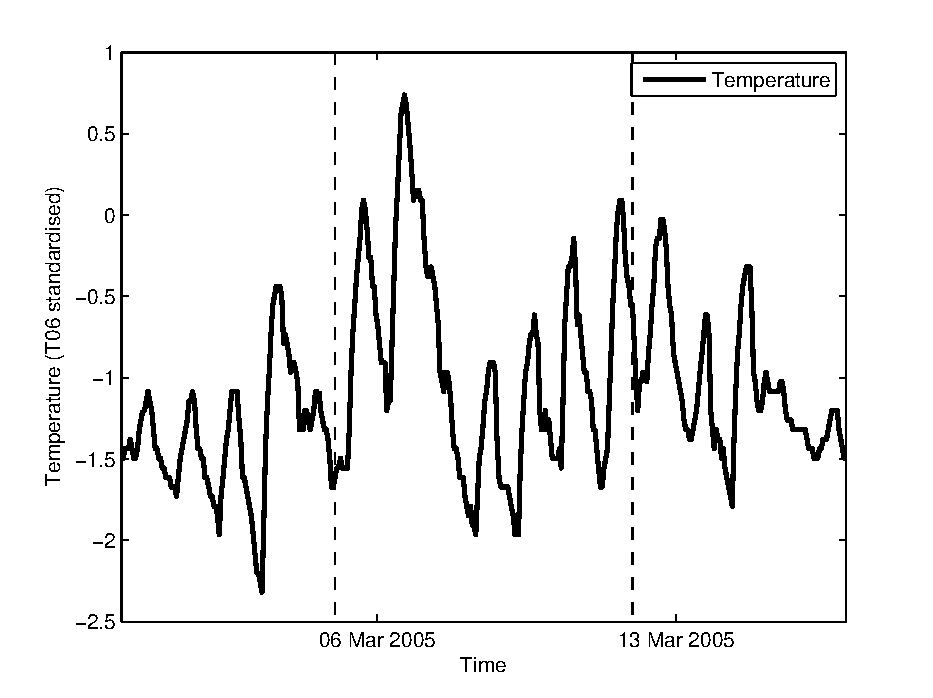
\includegraphics[width=0.5\textwidth]{../include/best_temp.pdf}
    };
  \end{scope}
\end{tikzpicture}

%  \end{center}
%\end{frame}
%
%\begin{frame}{GP regression - without structure}
%  \vspace{-1\baselineskip}
%    \begin{eqnarray*}
%    \textrm{Load} & = & \textrm{Smooth function of time}
%  \end{eqnarray*}
%  \begin{center}
%    \begin{tikzpicture}
  \begin{scope}[xshift=0cm]
    \node [mybox] (box){
      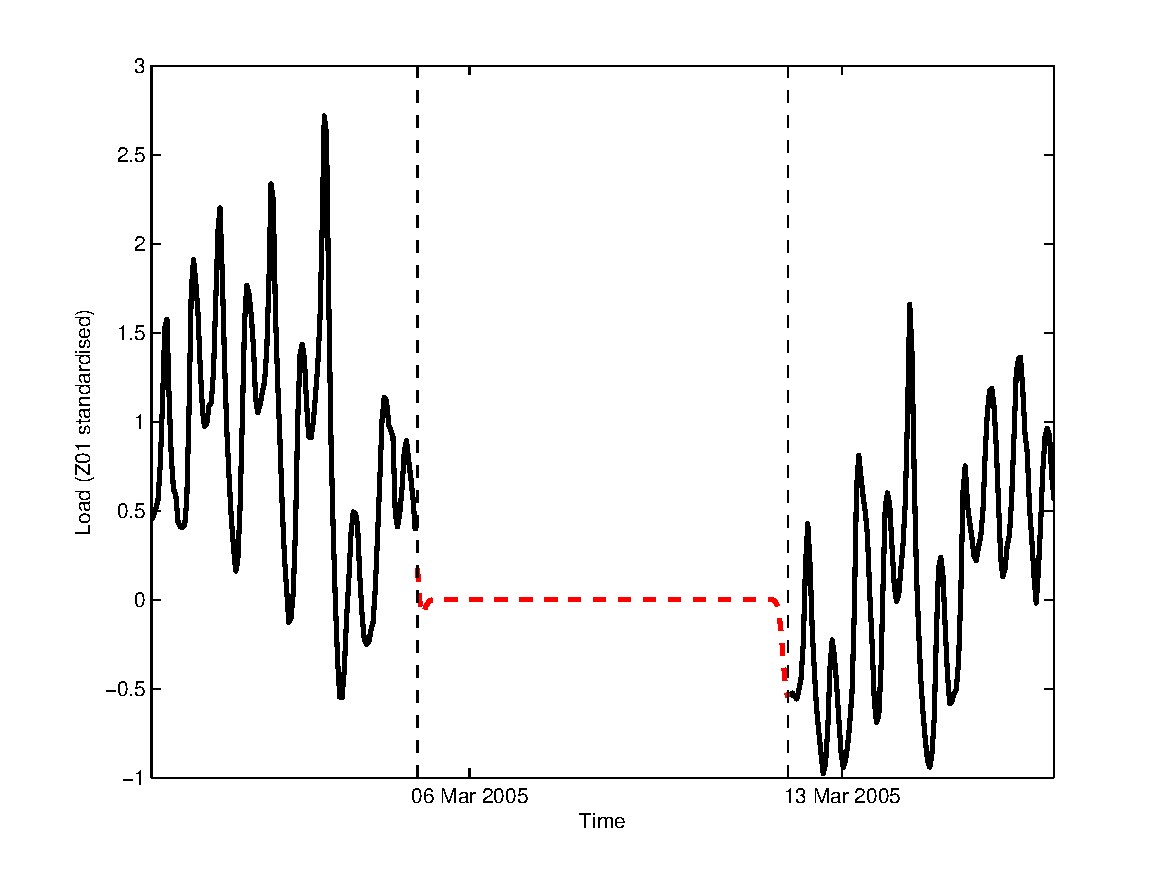
\includegraphics[width=0.5\textwidth]{../include/load_pred_SE.pdf}
    };
  \end{scope}
  \begin{scope}[xshift=0.5\textwidth]
    \node [mybox] (box){
      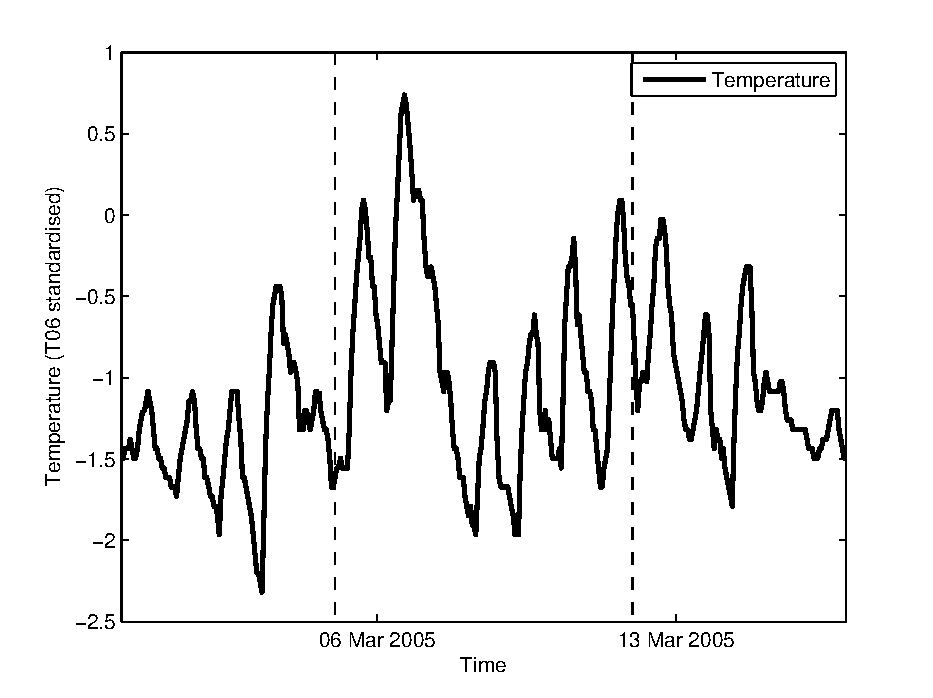
\includegraphics[width=0.5\textwidth]{../include/best_temp.pdf}
    };
  \end{scope}
\end{tikzpicture}

%  \end{center}
%  Suitable prior assumptions crucial when using any Bayesian method
%\end{frame}

\begin{frame}{Structured kernels for temp.\ forecasts}
  %\begin{itemize}
  %  \item Assumed that Temperature = Smoothed historical average + Smooth long-term deviations + Daily periodicity
  %\end{itemize}
  \begin{eqnarray*}
    \textrm{Temperature} & = & \textrm{Smooth historical average temperature} +  \\
    & & \textrm{Smooth long-term deviations} + \\
    & & \textrm{Daily periodicity}
  \end{eqnarray*}
  \begin{center}
    \begin{tikzpicture}
  \begin{scope}[xshift=0cm]
    \node [mybox] (box){
      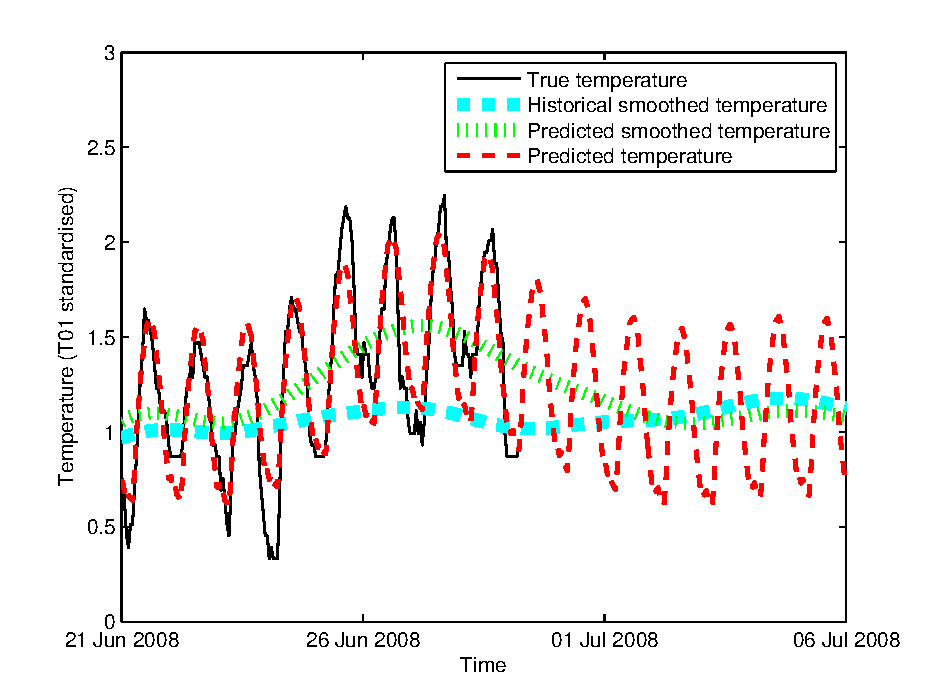
\includegraphics[width=0.7\textwidth]{../include/temp_pred.pdf}
    };
  \end{scope}
\end{tikzpicture}

  \end{center}
\end{frame}

\begin{frame}{GP regression - parameter selection}
  \begin{itemize}
    \item Can optimise marginal likelihood (a balance of model fit and complexity) with gradient based optimisation
    \vspace{\baselineskip}
    \item Marginal likelihood optimisation can fail
    \begin{itemize}
      \item Can result in slight over fitting
      \item When the prior and data generation process are dissimilar, Bayesian inference can give misleading results
    \end{itemize}
    \vspace{\baselineskip}
    \item In practice, parameter selection was a mixture of marginal likelihood optimisation, validation score maximisation and model checking (plotting graphs)
  \end{itemize}
\end{frame}

\begin{frame}{Competition inspired new GP research}
  \begin{itemize}
    \item Creating custom composite kernels not a new idea, but typically only practised by GP / kernel learning experts
    \vspace{\baselineskip}
    \item After competition, automated the process of kernel / model construction \cite{duvenaud2013structure} based on an idea by \cite{Grosse2012} in the context of matrix factorisation
    \vspace{\baselineskip}
    \item Ongoing research to see how far the automatic model construction idea can be pushed \eg
  \end{itemize}
  \begin{tabular}{ccc}
\hspace{-0.5cm}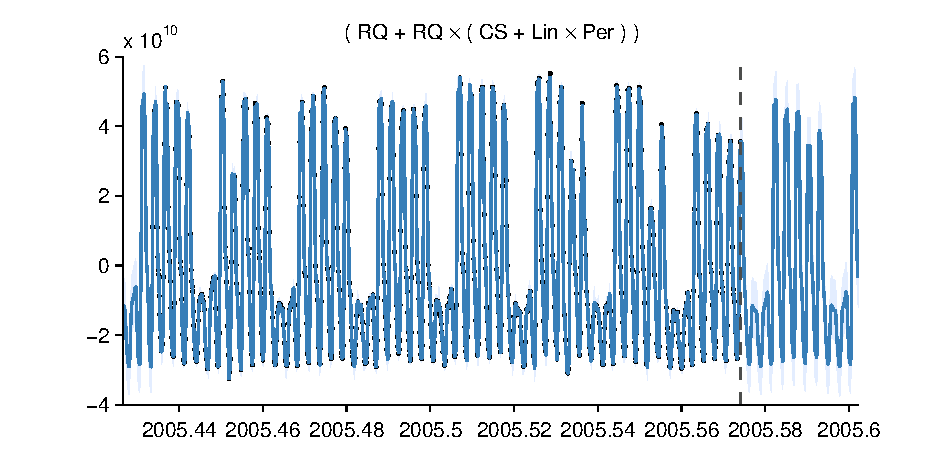
\includegraphics[width=0.33\textwidth]{figures/internet-traffic-data-in-bits-fr/internet-traffic-data-in-bits-fr_all} &
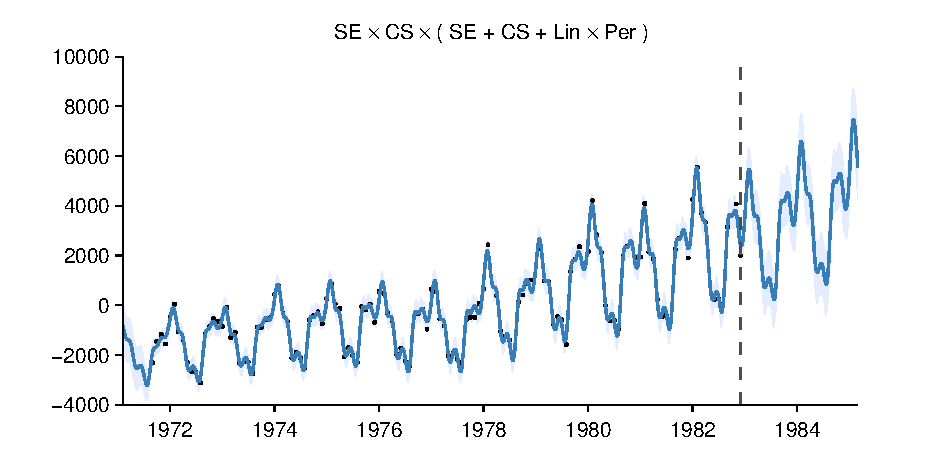
\includegraphics[width=0.32\textwidth]{figures/weekday-bus-ridership-iowa-city-/weekday-bus-ridership-iowa-city-_all} & 
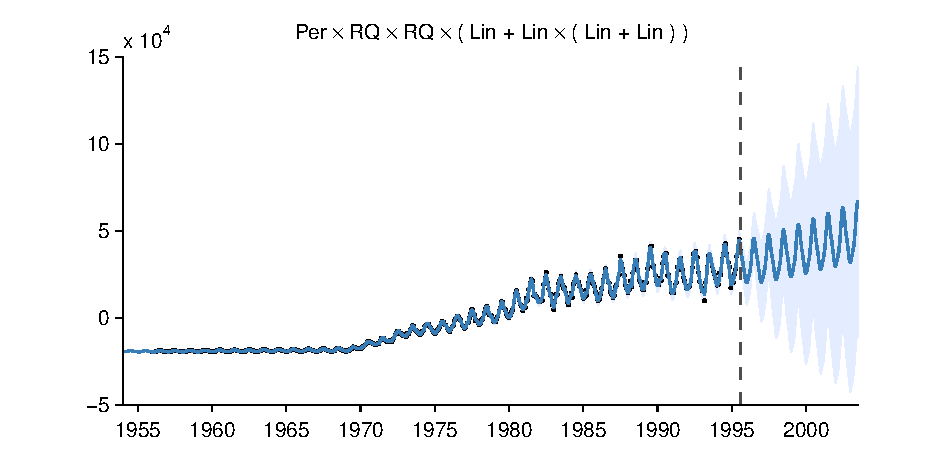
\includegraphics[width=0.32\textwidth]{figures/monthly-production-of-gas-in-aus/monthly-production-of-gas-in-aus_all} \\
\hspace{-0.5cm}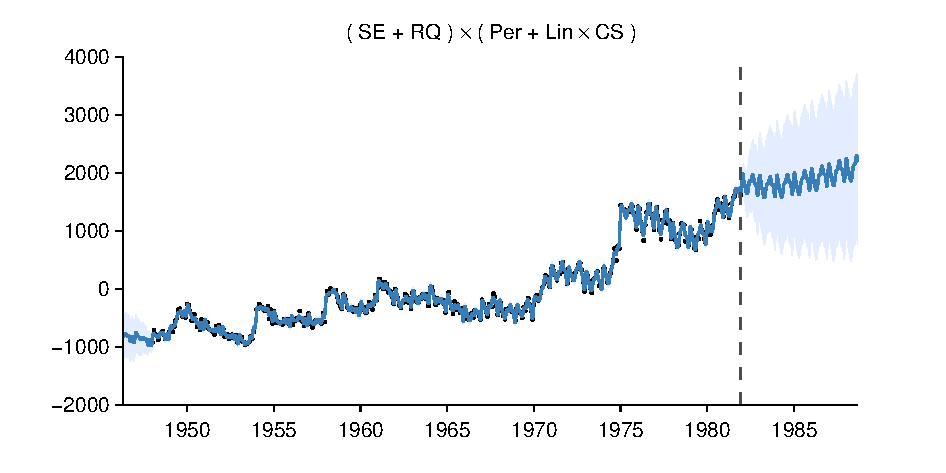
\includegraphics[width=0.33\textwidth]{figures/monthly-us-female-20-years-and-o/monthly-us-female-20-years-and-o_all} &
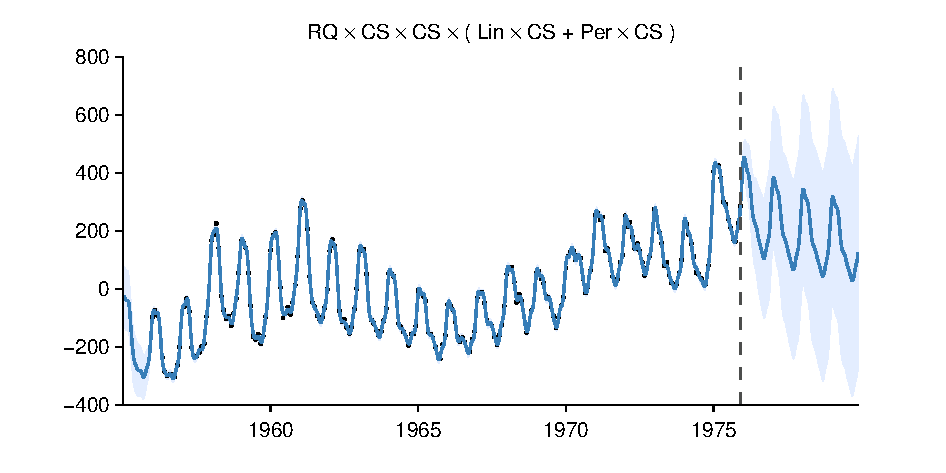
\includegraphics[width=0.32\textwidth]{figures/monthly-canadian-total-unemploym/monthly-canadian-total-unemploym_all} & 
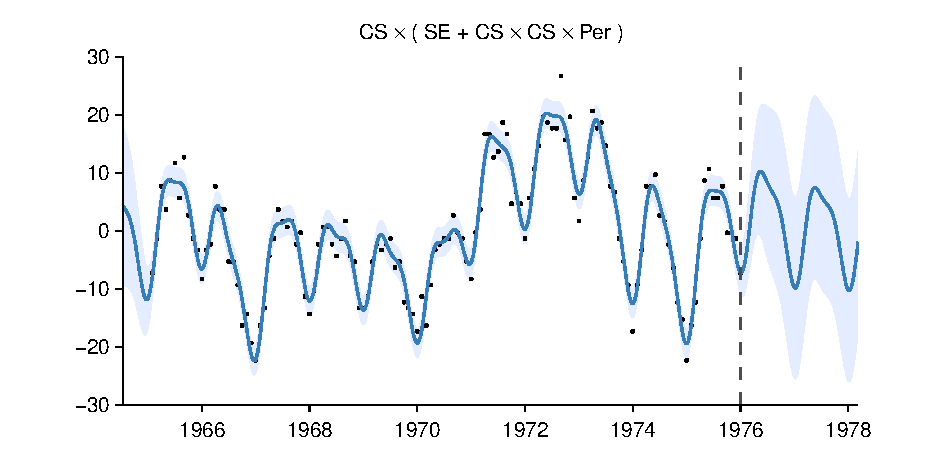
\includegraphics[width=0.32\textwidth]{figures/monthly-sales-of-us-houses-thous/monthly-sales-of-us-houses-thous_all}
  \end{tabular}
\end{frame}

\begin{frame}{Ensembling}
  \begin{block}{Small search over possible weightings}
    \begin{center}
      \scriptsize
      \begin{tabular}{cccc|c}
        GBM & GP & RF & LM & Score \\
        \hline
        100 & 0 & 0 & 0 & 72,968 \\
        0 & 100 & 0 & 0 & 99,787 \\
        0 & 0 & 100 & 0 & 89,457 \\
        0 & 0 & 0 & 100 & 112,547 \\
        80 & 20 & 0 & 0 & 71,683 \\
        70 & 30 & 0 & 0 & 72,485 \\
        90 & 10 & 0 & 0 & 71,846 \\
        85 & 15 & 0 & 0 & 71,644 \\
        \bf{76} & \bf{14} & \bf{0} & \bf{10} & \bf{71,164} \\
        72 & 13 & 10 & 5 & 71,566 \\
        80 & 0 & 20 & 10 & 74,293 \\
        \ldots & \ldots & \ldots & \ldots & \ldots
      \end{tabular}
      \vspace{-1\baselineskip}
    \end{center}
      \vspace{-1\baselineskip}
  \end{block}
  \begin{block}{More principled methods}
    \begin{itemize}
      \item Grid searches and cross validation - but could be costly to retrain algorithms on different training / test splits
      \item Bayesian optimisation \cite{Osborne2009}, \cite{snoek2012practical}, \cite{HennigSchuler2012} can be more appropriate when individual evaluations costly (\eg submitting to Kaggle to obtain validation score)
    \end{itemize}
  \end{block}
\end{frame}

\begin{frame}{Summary}
  \begin{itemize}
    \item Main approach was to regress loads on time and temperature, rather than using an autoregressive model
    \vspace{2\baselineskip}
    \item GBM provided the majority of performance
    \vspace{2\baselineskip}
    \item Structured kernel GP method sufficiently uncorrelated to provide useful component in ensemble
  \end{itemize}
\end{frame}

{
\section{References}
\section{Extended Bibliography}
\tiny
\begin{frame}[allowframebreaks,plain]
  \frametitle{References}
  \bibliography{library}
  \bibliographystyle{alpha}
\end{frame}
}

\end{document}